% !TEX program = xelatex
\documentclass[a4paper]{exam}
\usepackage{amsmath}
\usepackage{amsthm}
\usepackage[left=1.8cm,right=1.8cm,top=2.2cm,bottom=2.0cm]{geometry}
\usepackage[UTF8]{ctex}
\usepackage{enumerate}
\usepackage{fancyhdr}
\usepackage{xpatch}
\usepackage{graphicx} 
\usepackage{float} 
\usepackage{subfigure} 
\usepackage{amsfonts}
\usepackage{mathtools}
\usepackage{framed}
\usepackage{multicol}
\usepackage{minted}
\usepackage{fontspec}
\usepackage{float}
\usepackage{tikz}
\usepackage{multicol,comment}
\usepackage{biblatex}
\addbibresource{05-discussion.bib}
\usepackage{tikz}

\usetikzlibrary{automata,positioning}
\theoremstyle{definition}
\newtheorem*{solution*}{\textbf{Solution:}}
\newtheorem*{proof*}{\textbf{Proof:}}
\newtheorem{theorem}{Theorem}[subsection]
\newtheorem{definition}{Definition}[subsection]
\newtheorem{lemma}{Lemma}[subsection]
\makeatletter

\AtBeginDocument{\xpatchcmd{\@thm}{\thm@headpunct{.}}{\thm@headpunct{}}{}{}}
\makeatother

\pagestyle{fancy}
\renewcommand{\baselinestretch}{1.15}

\usepackage{paralist}
\let\itemize\compactitem
\let\enditemize\endcompactitem
\let\enumerate\compactenum
\let\endenumerate\endcompactenum
\let\description\compactdesc
\let\enddescription\endcompactdesc

% shorten footnote rule
\xpatchcmd\footnoterule
  {.4\columnwidth}
  {1in}
  {}{\fail}

\title{CS 131 Compilers: Discussion 5: Intermediate Representation}
\author{\textbf{杨易为}~~\textbf{吴凌云}~~\textbf{樊雨鑫} \\ \texttt{ \{yangyw,wuly2,fanyx\}@shanghaitech.edu.cn}}


\begin{document}
\maketitle
\section{Intermediate Representations}
An Intermediate Representation (IR) is an intermediate (neither source nor target) form of a program. There are various types of IRs:
\begin{enumerate}
  \item Section
        \begin{enumerate}
          \item \textbf{Abstract Syntax Trees} (AST): a simplified Parse Tree.\\
                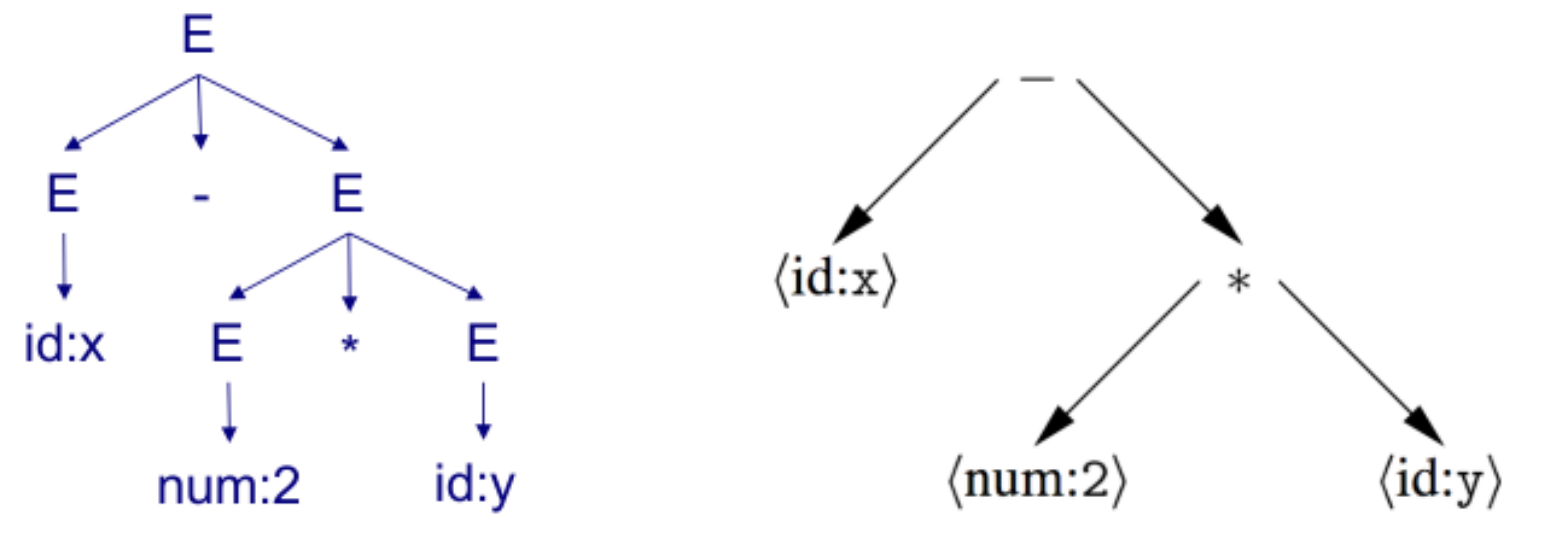
\includegraphics[width=10cm]{img/ast.png}
                \begin{itemize}
                  \item + close to source compactdesc
                  \item + suitable for source-source translation
                  \item - Traversal \& Transformations are expensive
                  \item - Pointer-intensive
                  \item - Memory-allocation-intensive
                \end{itemize}

          \item \textbf{Directed Acyclic Graphs} (DAG): DAG is an optimized AST, with identical nodes \textit{shared}.\\
                \begin{figure}[htbp]
                  \centering
                  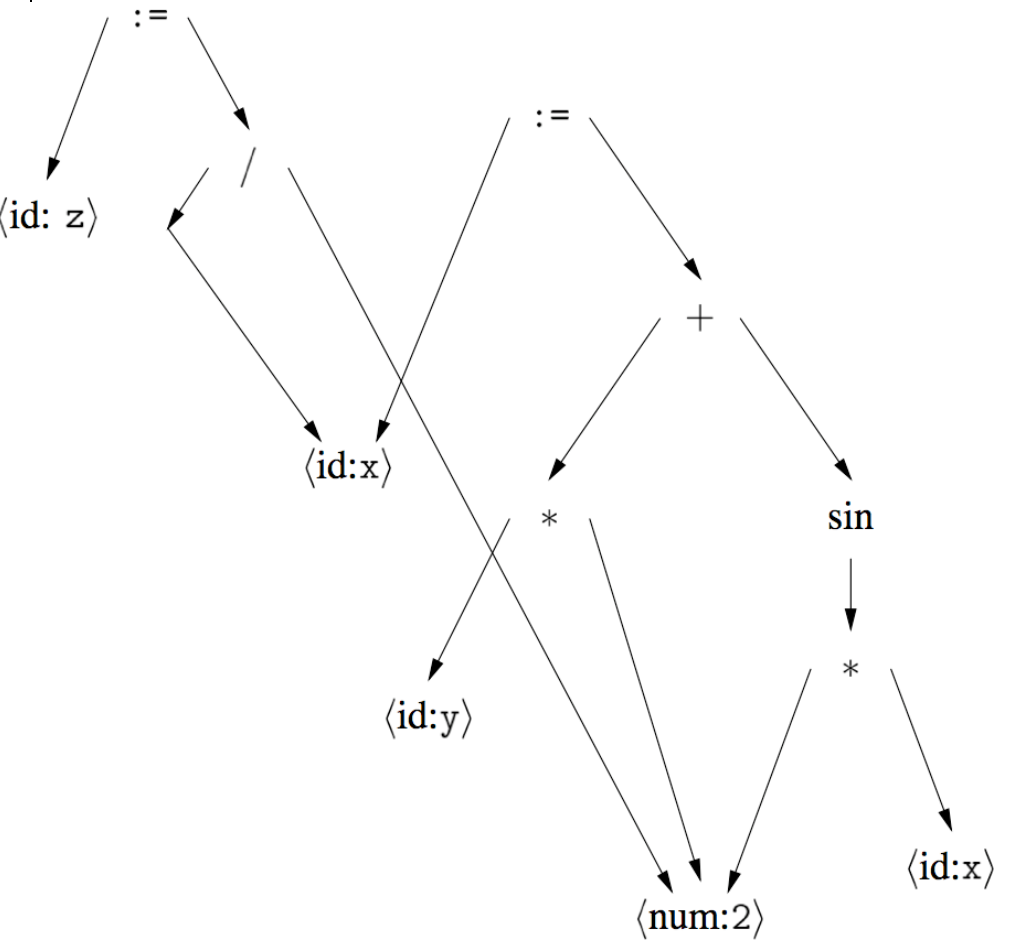
\includegraphics[width=6cm]{img/dag.png}
                \end{figure}
                \begin{itemize}
                  \item + Explicit sharing
                  \item + Exposes redundancy, more efficient, useful for dynamic pipelining analysis
                  \item - Difficult to transform
                  \item - Analysis usage Practical usage
                \end{itemize}
          \item \textbf{Control Flow Graphs} (CFG): CFG is a flow chart of program execution. Is a conservative approximation of the Control Flow, because only one branch will be actually executed.\\
                A Basic Block is a consecutive sequence of Statements $S_{1}, \ldots, S_{n}$, where flow must enter this block only at $S_{1}$, AND if $S_{1}$ is executed, then $S_{2}, \ldots, S_{n}$ are executed strictly in that order, unless one Statement causes halting.

                \begin{itemize}
                  \item The Leader is the first Statement of a Basic Block
                  \item A Maximal Basic Block is a maximal-length Basic Block
                \end{itemize}
                Nodes of a CFG are Maximal Basic Blocks, and Edges of a CFG represent control flows
                \begin{itemize}
                  \item $\exists$ edge $b_{1} \rightarrow b_{2}$ iff control may transfer from the last Statement of $b_{1}$ to the first Statement of $b_{2}$
                \end{itemize}
                \begin{figure}[htbp]
                  \centering
                  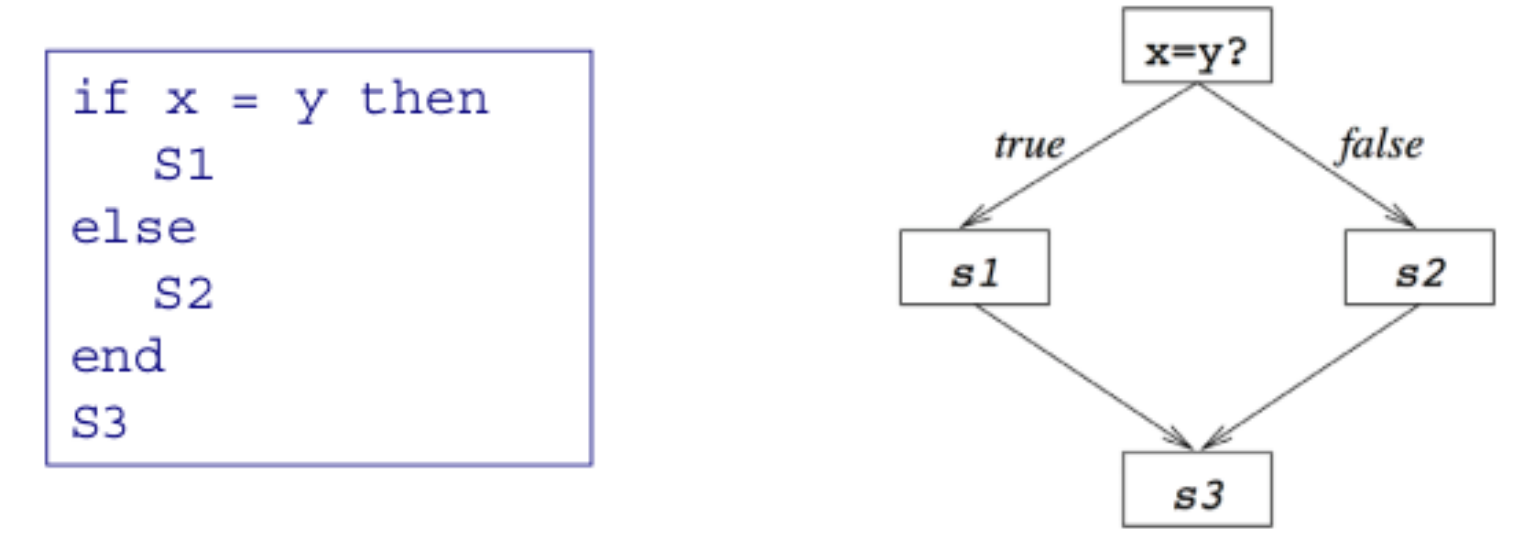
\includegraphics[width=6cm]{img/if_cfg_bb.png}
                \end{figure}
                \begin{itemize}
                  \item + Most widely used form. Can cast static analysis\cite{njuswanalysis} on it.
                \end{itemize}
          \item \textbf{Single Static Assignment} (SSA): SSA means every variable will only be assigned value ONCE (therefore single). Useful for various kinds of optimizations.\\
                \begin{figure}[htbp]
                  \centering
                  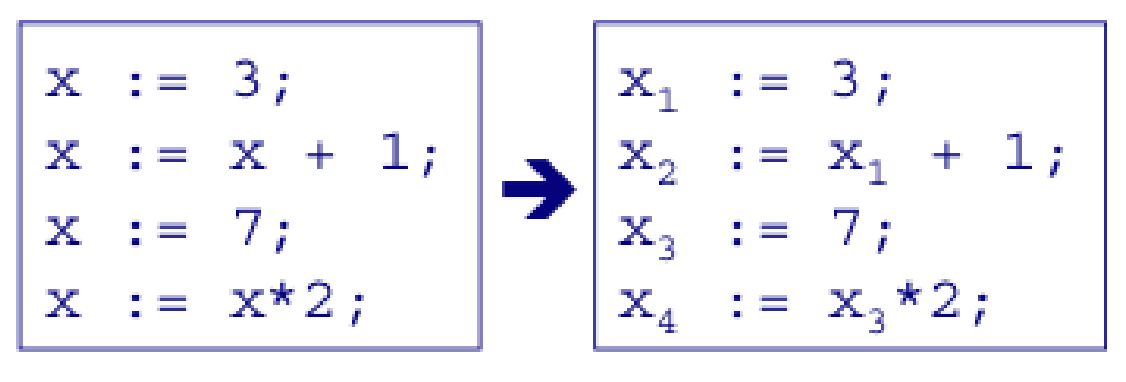
\includegraphics[width=6cm]{img/ssa_rename.png}
                \end{figure}
                A $\phi$ -function generates an extra assignment to "choose" from Branches or Loops. If Basic Block $B$ has Predecessors $P_{1}, \ldots, P_{n}$, then $X=\phi\left(v_{1}, \ldots, v_{n}\right)$ assigns $X=v_{j}$ if control enters $B$ from $P_{j}$.\\
                \begin{figure}[htbp]
                  \centering
                  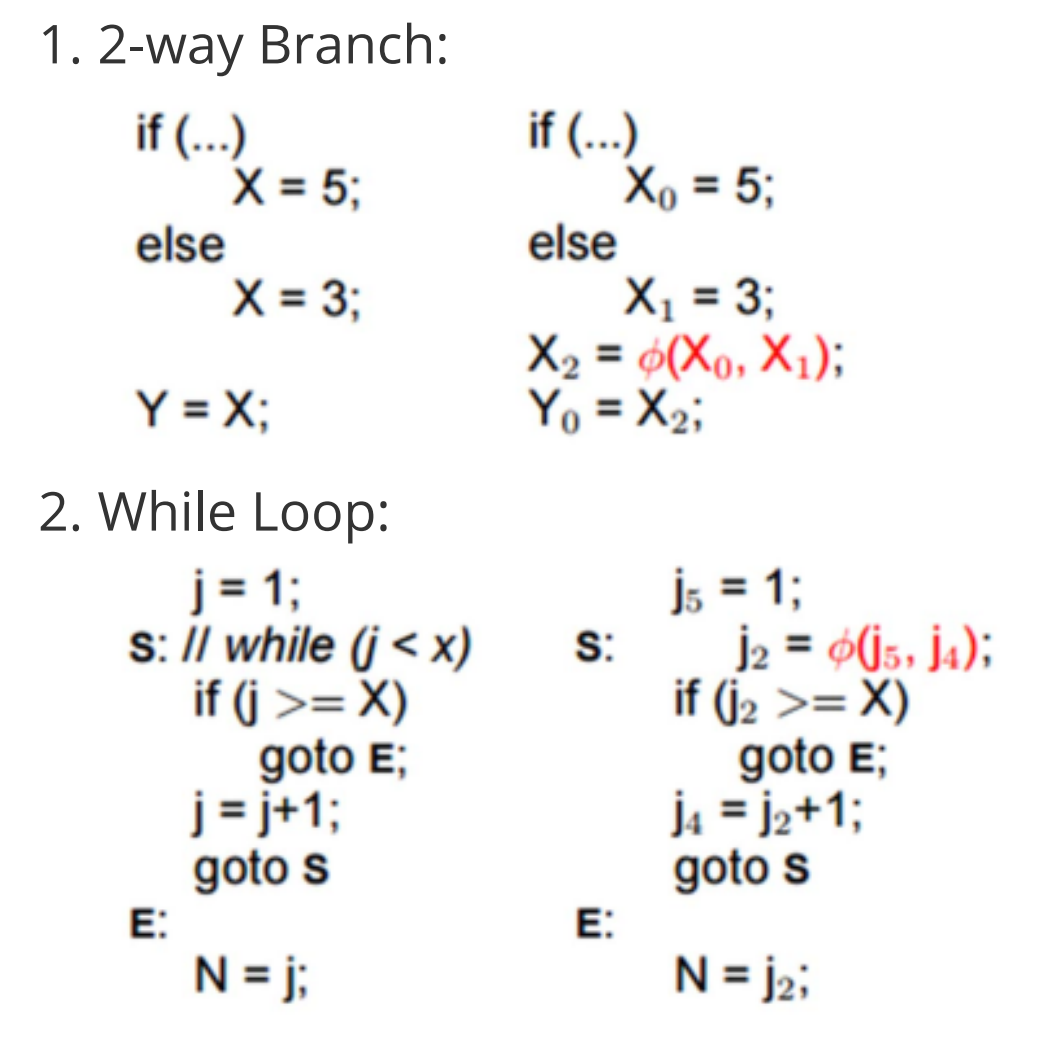
\includegraphics[width=6cm]{img/insert_phi.png}
                \end{figure}
                \begin{enumerate}
                  \item $\phi$ is not an executable operation
                  \item Number of $\phi$ arguments $=$ Number of incoming edges
                  \item Where to place a $\phi ?$ If Basic Block $B$ contains an assignment to variable $X$, then a $\phi$ MUST be inserted before each Basic Block $Z$ that:\\
                        1. $\exists$ non-empty path $B \rightarrow^{+} Z$\\
                        2. $\exists$ path from ENTRY to $Z$ which does not go through $B$\\
                        3. $Z$ is the FIRST node that satisfies $\mathrm{i}$. and ii.
                \end{enumerate}
        \end{enumerate}
\end{enumerate}
\subsection{$\phi$ Function insertion in Light IR}
% TODO
\subsection{Reusable IR\cite{llvmintro}}
\begin{enumerate}
  \item Modern compilers are made from loosely coupled components.
  \item Front ends produce IR, AST as well. Thus they have to maintain all the information on Basic Block.
  \item Middle 'ends' transform IR (optimization / analysis / instrumentation)
  \item Back ends generate native code (object code or assembly)
\end{enumerate}

\begin{center}
  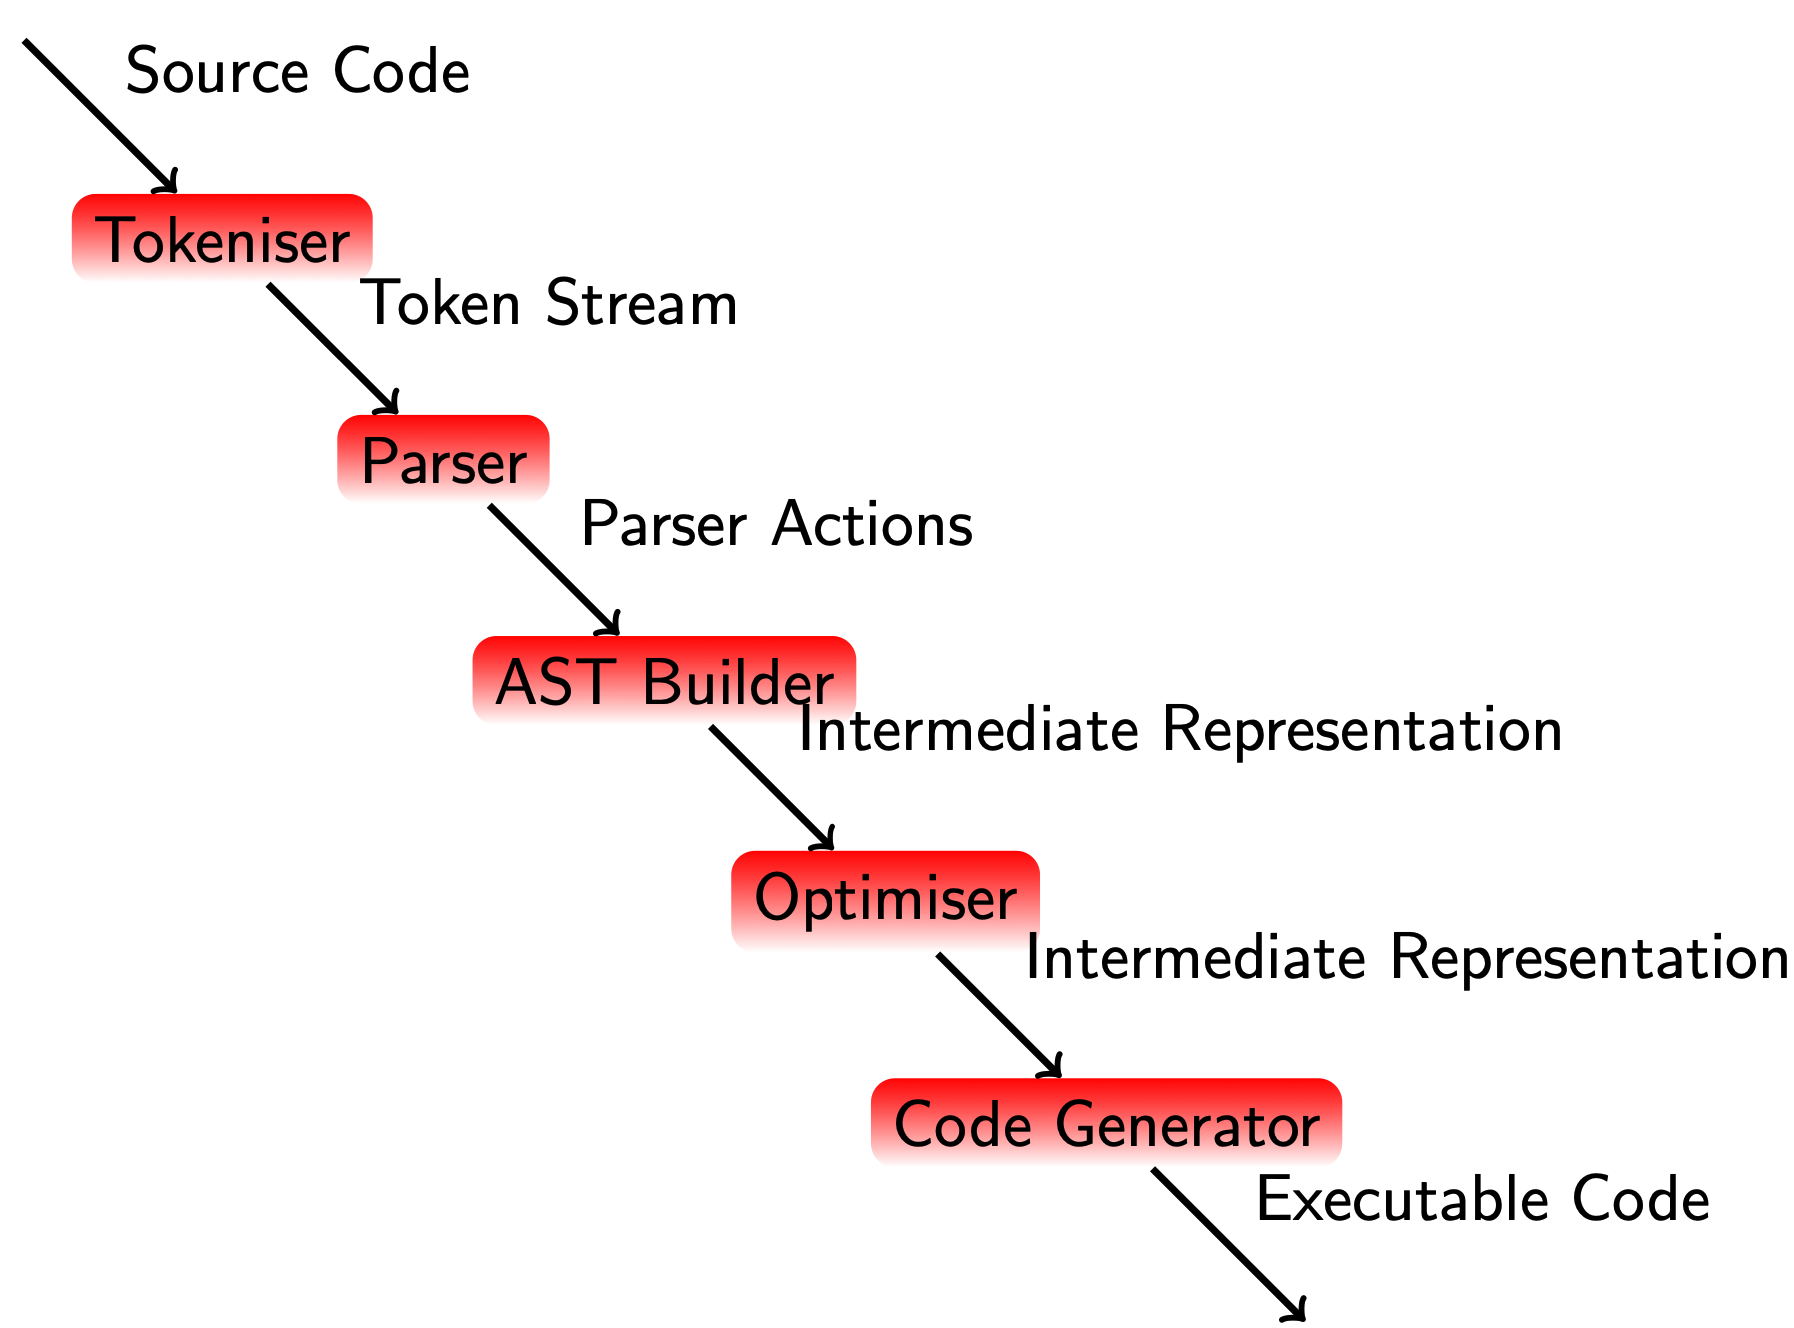
\includegraphics[height=3cm]{img/llvm.png}
\end{center}

As with any other piece of software using libraries simplifies development.

\subsection{Optimization Passes}
\begin{enumerate}
  \item  Modular, transform IR (Analysis passes just inspect IR)
  \item Can be run multiple times, in different orders
  \item May not always produce improvements when run in the wrong order!
  \item Some intentionally pessimistic code to make later passes work better
\end{enumerate}

\subsection{Register vs Stack IR}
\begin{enumerate}
  \item Stack makes interpreting, naive compilation easier • Register makes various optimizations easier
  \item Which ones?
\end{enumerate}
  \begin{figure}[h]
    \centering
    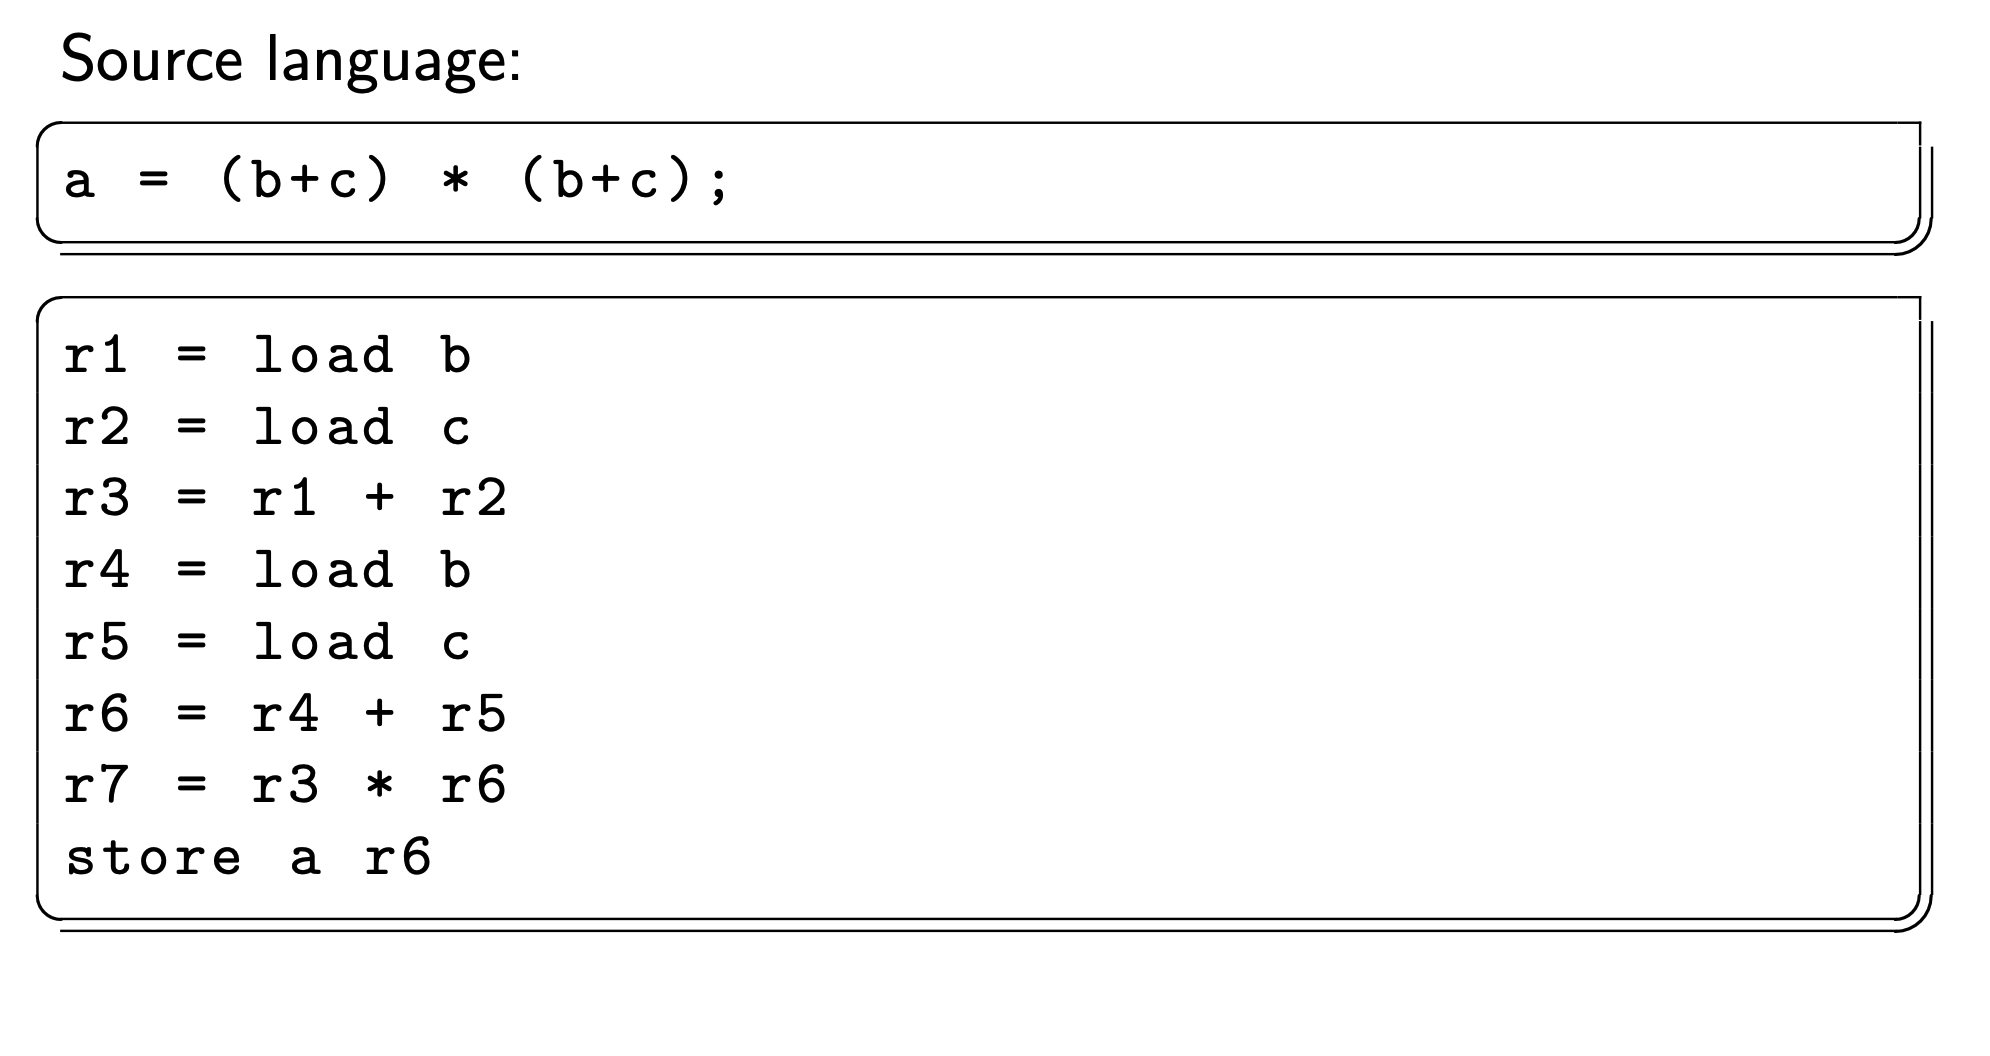
\includegraphics[height=3cm]{img/Snipaste_2021-04-05_17-25-13.png}
    \caption{Registers}
  \end{figure}

  \begin{figure}[h]
    \centering
    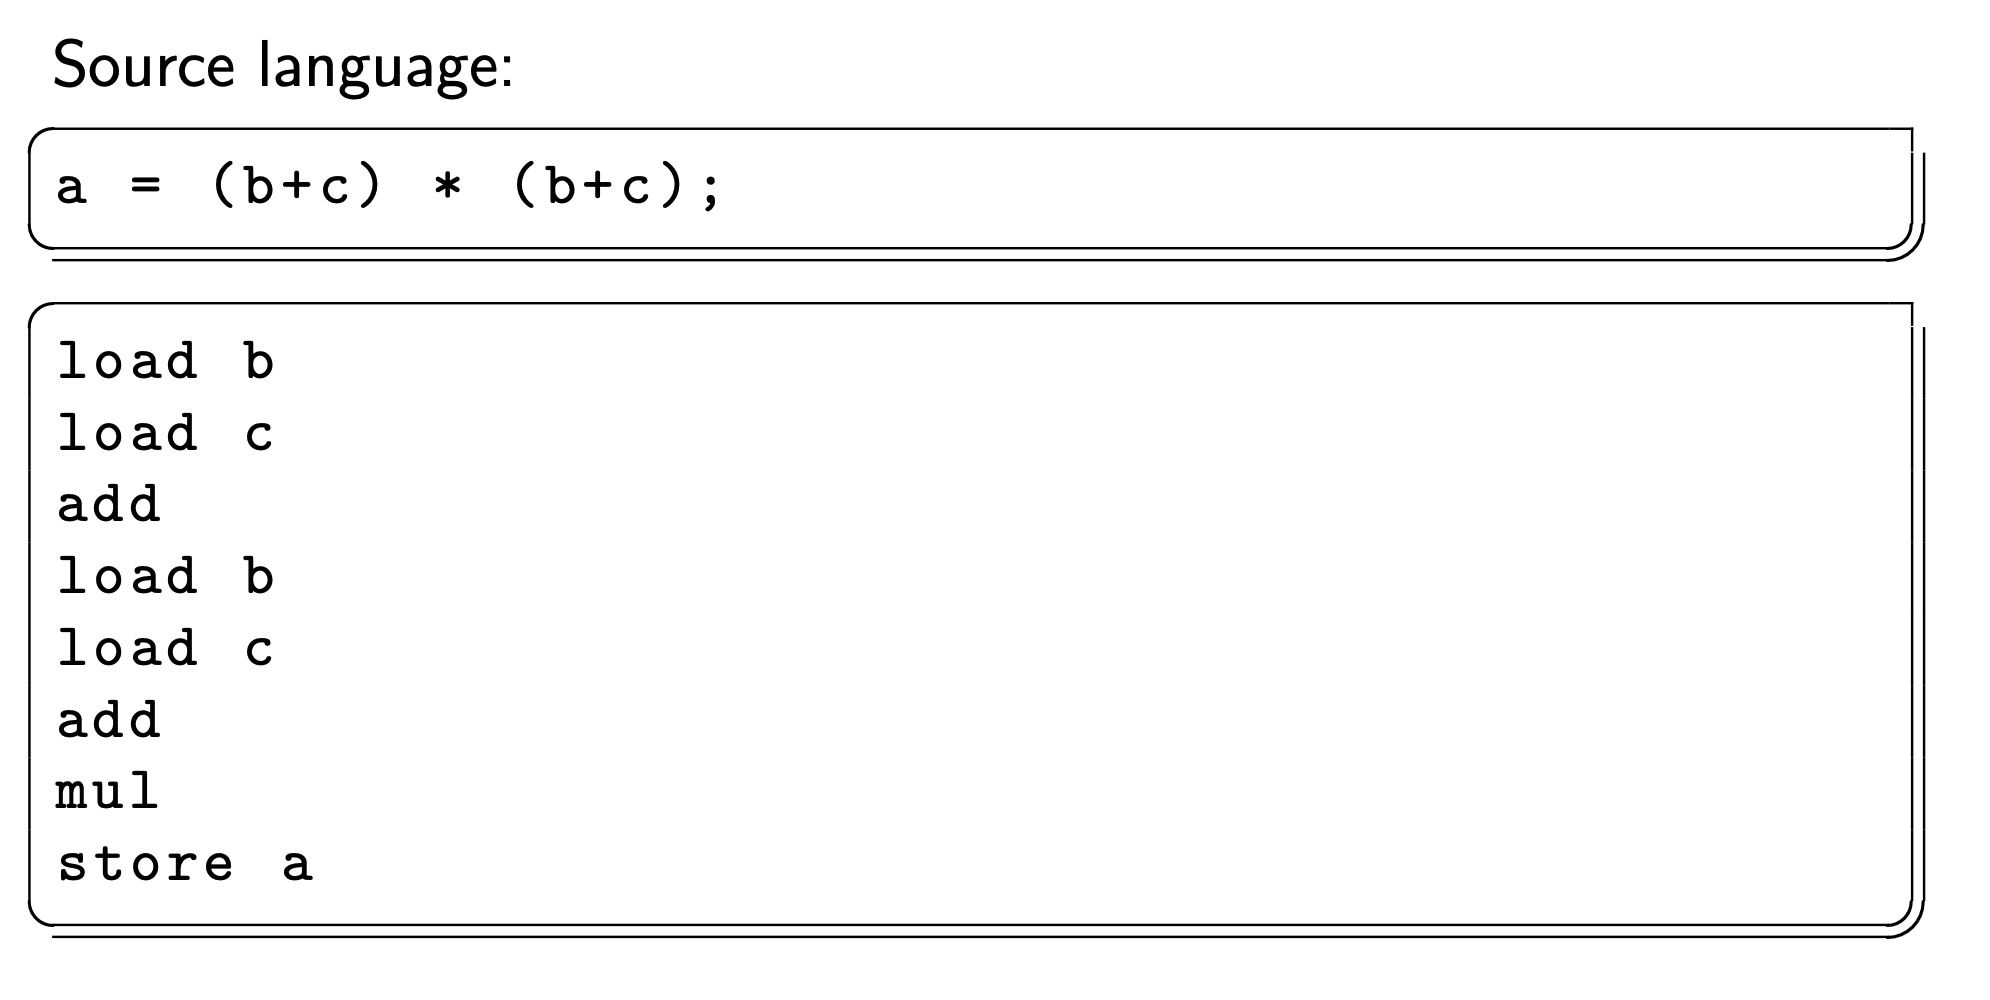
\includegraphics[height=3cm]{img/source_example.png}
    \caption{Stack IR}
  \end{figure}
\subsubsection{Problems with CSE and Stack IR}

\begin{enumerate}
  \item Entire operation must happen at once (no incremental algorithm)
  \item Finding identical subtrees is possible, reusing results is harder • If the operations were not adjacent, must spill to temporary
\end{enumerate}

\subsubsection{Hierarchical vs Flat IR}
\begin{enumerate}
  \item Source code is hierarchical (contains structured flow control, scoped values)
  \item Assembly is flat (all flow control is by jumps)
  \item Intermediate representations are supposed to be somewhere
        between the two
  \item Think about the possible ways that a for loop, while loop, and if statement with a backwards goto might be represented.
\end{enumerate}

\subsubsection{Hierarchical IR}
\begin{enumerate}
  \item  Easy to express high-level constructs
  \item Preserves program semantics
  \item Preserves high-level semantics (variable lifetime, exceptions) clearly
  \item Example: Ark Compiler, Flamming my compiler
\end{enumerate}
\subsection{Flat IR}

\begin{enumerate}
  \item Easy to map to the back end
  \item Simple for optimizations to process
  \item Must carry scope information in ad-hoc ways (e.g. LLVM IR has intrinsics to explicitly manage lifetimes for stack allocations)
  \item Examples: LLVM IR, CGIR, PTX
\end{enumerate}
\section{What Is LLVM IR?}
\begin{enumerate}
  \item Unlimited Single-Assignment Register machine instruction set • Strongly typed
  \item Three common representations:
  \item Human-readable LLVM assembly (.ll files)
  \item Dense 'bitcode' binary representation (.bc files) • C++ classes
\end{enumerate}

\subsection{Unlimited Register Machine?}

\begin{enumerate}
  \item  Real CPUs have a fixed number of registers
  \item LLVM IR has an infinite number
  \item New registers are created to hold the result of every instruction
  \item CodeGen's register allocator determines the mapping from LLVM registers to physical registers
  \item Type legalization maps LLVM types to machine types and so on (e.g. 128-element float vector to 32 SSE vectors or 16 AVX vectors, 1-bit integers to 32-bit values)
\end{enumerate}

\subsection{Static Single Assignment}
\begin{enumerate}
  \item Registers may be assigned to only once
  \item Most (imperative) languages allow variables to be... variable
  \item This requires some e↵ort to support in LLVM IR: SSA registers are not variables
  \item SSA form makes dataflow explicit: All consumers of the result of an instruction read the output register(s)
\end{enumerate}

\textbf{Example:}
\begin{minted}[mathescape, linenos]{c}
int a = someFunc();
a++;
\end{minted}
One variable, assigned to twice.
\begin{minted}[mathescape, linenos]{llvm}
%a = call i32 @someFunc()
%a = add i32 %a, 1
\end{minted}
error: multiple definition of local value named 'a'\\
\texttt{\%a = \$add i32 \%a, 1}
\begin{enumerate}
  \item Front end must keep track of which register holds the current value of a at any point in the code
  \item How do we track the new values?
\end{enumerate}
\subsection{Translating to LLVM IR The Easy Way}
\begin{minted}[mathescape, linenos]{llvm}
; int a
%a = alloca i32, align 4
; a = someFunc
%0 = call i32 @someFunc()
store i32 %0, i32* %0, a
; a++
%1 = load i32* %a
%2 = add i32 %1, 1
store i32 %2, i32* %a
\end{minted}
\begin{enumerate}
  \item Numbered register are allocated automatically
  \item  Each expression in the source is translated without worrying
        about data flow
  \item  Memory is not SSA in LLVM
\end{enumerate}
\subsubsection{Isn't That Slow?}
\begin{enumerate}
  \item Lots of redundant memory operations
  \item Stores followed immediately by loads
  \item The Scalar Replacement of Aggregates (SROA) or mem2reg pass cleans it up for us.
  \item But SROA only works if the \texttt{alloca} is declared in the entry block to the function!
\end{enumerate}
\begin{minted}[mathescape, linenos]{llvm}
%0 = call i32 @someFunc()
%1 = add i32 %0, 1
\end{minted}
\subsubsection{Mem2Reg}
This file promotes memory references to be register references. It promotes alloca instructions which only have loads and stores as uses. An alloca is transformed by using dominator frontiers to place phi nodes, then traversing the function in depth-first order to rewrite loads and stores as appropriate. This is just the standard SSA construction algorithm to construct "pruned" SSA form.

\begin{minted}[mathescape, linenos]{llvm}
  ; RUN: opt < %s -instcombine -mem2reg -S | grep "%A = alloca" 
  ; RUN: opt < %s -instcombine -mem2reg -S | \
  ; RUN:    not grep "%B = alloca"
  ; END.
  
  ; Ensure that instcombine doesn't sink the loads in entry/cond_true into 
  ; cond_next.  Doing so prevents mem2reg from promoting the B alloca.
  
  define i32 @test2(i32 %C) {
  entry:
    %A = alloca i32
    %B = alloca i32
    %tmp = call i32 (...) @bar( i32* %A ); <i32> [#uses=0]
    %T = load i32, i32* %A; <i32> [#uses=1]
    %tmp2 = icmp eq i32 %C, 0; <i1> [#uses=1]
    br i1 %tmp2, label %cond_next, label %cond_true
  
  cond_true:; preds = %entry
    store i32 123, i32* %B
    call i32 @test2( i32 123 ); <i32>:0 [#uses=0]
    %T1 = load i32, i32* %B; <i32> [#uses=1]
    br label %cond_next
  
  cond_next:; preds = %cond_true, %entry
    %tmp1.0 = phi i32 [ %T1, %cond_true ], [ %T, %entry ]; <i32> [#uses=1]
    %tmp7 = call i32 (...) @baq( ); <i32> [#uses=0]
    %tmp8 = call i32 (...) @baq( ); <i32> [#uses=0]
    %tmp9 = call i32 (...) @baq( ); <i32> [#uses=0]
    %tmp10 = call i32 (...) @baq( ); <i32> [#uses=0]
    %tmp11 = call i32 (...) @baq( ); <i32> [#uses=0]
    %tmp12 = call i32 (...) @baq( ); <i32> [#uses=0]
    %tmp13 = call i32 (...) @baq( ); <i32> [#uses=0]
    %tmp14 = call i32 (...) @baq( ); <i32> [#uses=0]
    %tmp15 = call i32 (...) @baq( ); <i32> [#uses=0]
    %tmp16 = call i32 (...) @baq( ); <i32> [#uses=0]
    %tmp17 = call i32 (...) @baq( ); <i32> [#uses=0]
    %tmp18 = call i32 (...) @baq( ); <i32> [#uses=0]
    %tmp19 = call i32 (...) @baq( ); <i32> [#uses=0]
    %tmp20 = call i32 (...) @baq( ); <i32> [#uses=0]
    ret i32 %tmp1.0
  }
  
  declare i32 @bar(...)
  
  declare i32 @baq(...)
\end{minted}
\subsection{Sequences of Instructions}
\begin{enumerate}

  \item A sequence of instructions that execute in order is a basic block
  \item Basic blocks must end with a terminator
  \item Terminators are intraprocedural flow control instructions.
  \item call is not a terminator because execution resumes at the same place after the call
  \item invoke is a terminator because flow either continues or branches to an exception cleanup handler
  \item This means that even “zero-cost” exceptions can have a cost: they complicate the control-flow graph (CFG) within a function and make optimization harder.
\end{enumerate}
\subsection{Intra-procedural Flow Control}
\begin{enumerate}
  \item Assembly languages typically manage flow control via jumps / branches (often the same instructions for inter- and intraprocedural flow)
  \item LLVM IR has conditional and unconditional branches
  \item Branch instructions are terminators (they go at the end of a
        basic block)
  \item Basic blocks are branch targets
  \item You can't jump into the middle of a basic block (by the definition of a basic block)
\end{enumerate}

\subsection{'Phi, my lord, phi!' - Lady Macbeth, Compiler Developer}

\begin{enumerate}
  \item  $\phi$ nodes are special instructions used in SSA construction
  \item Their value is determined by the preceding basic block
  \item $\phi$ nodes must come before any non- $\phi$ instructions in a basic
        block
  \item In code generation, $\phi$ nodes become a requirement for one
        basic block to leave a value in a specific register.
        Alternate representation: named parameters to basic blocks
\end{enumerate}
\begin{center}
  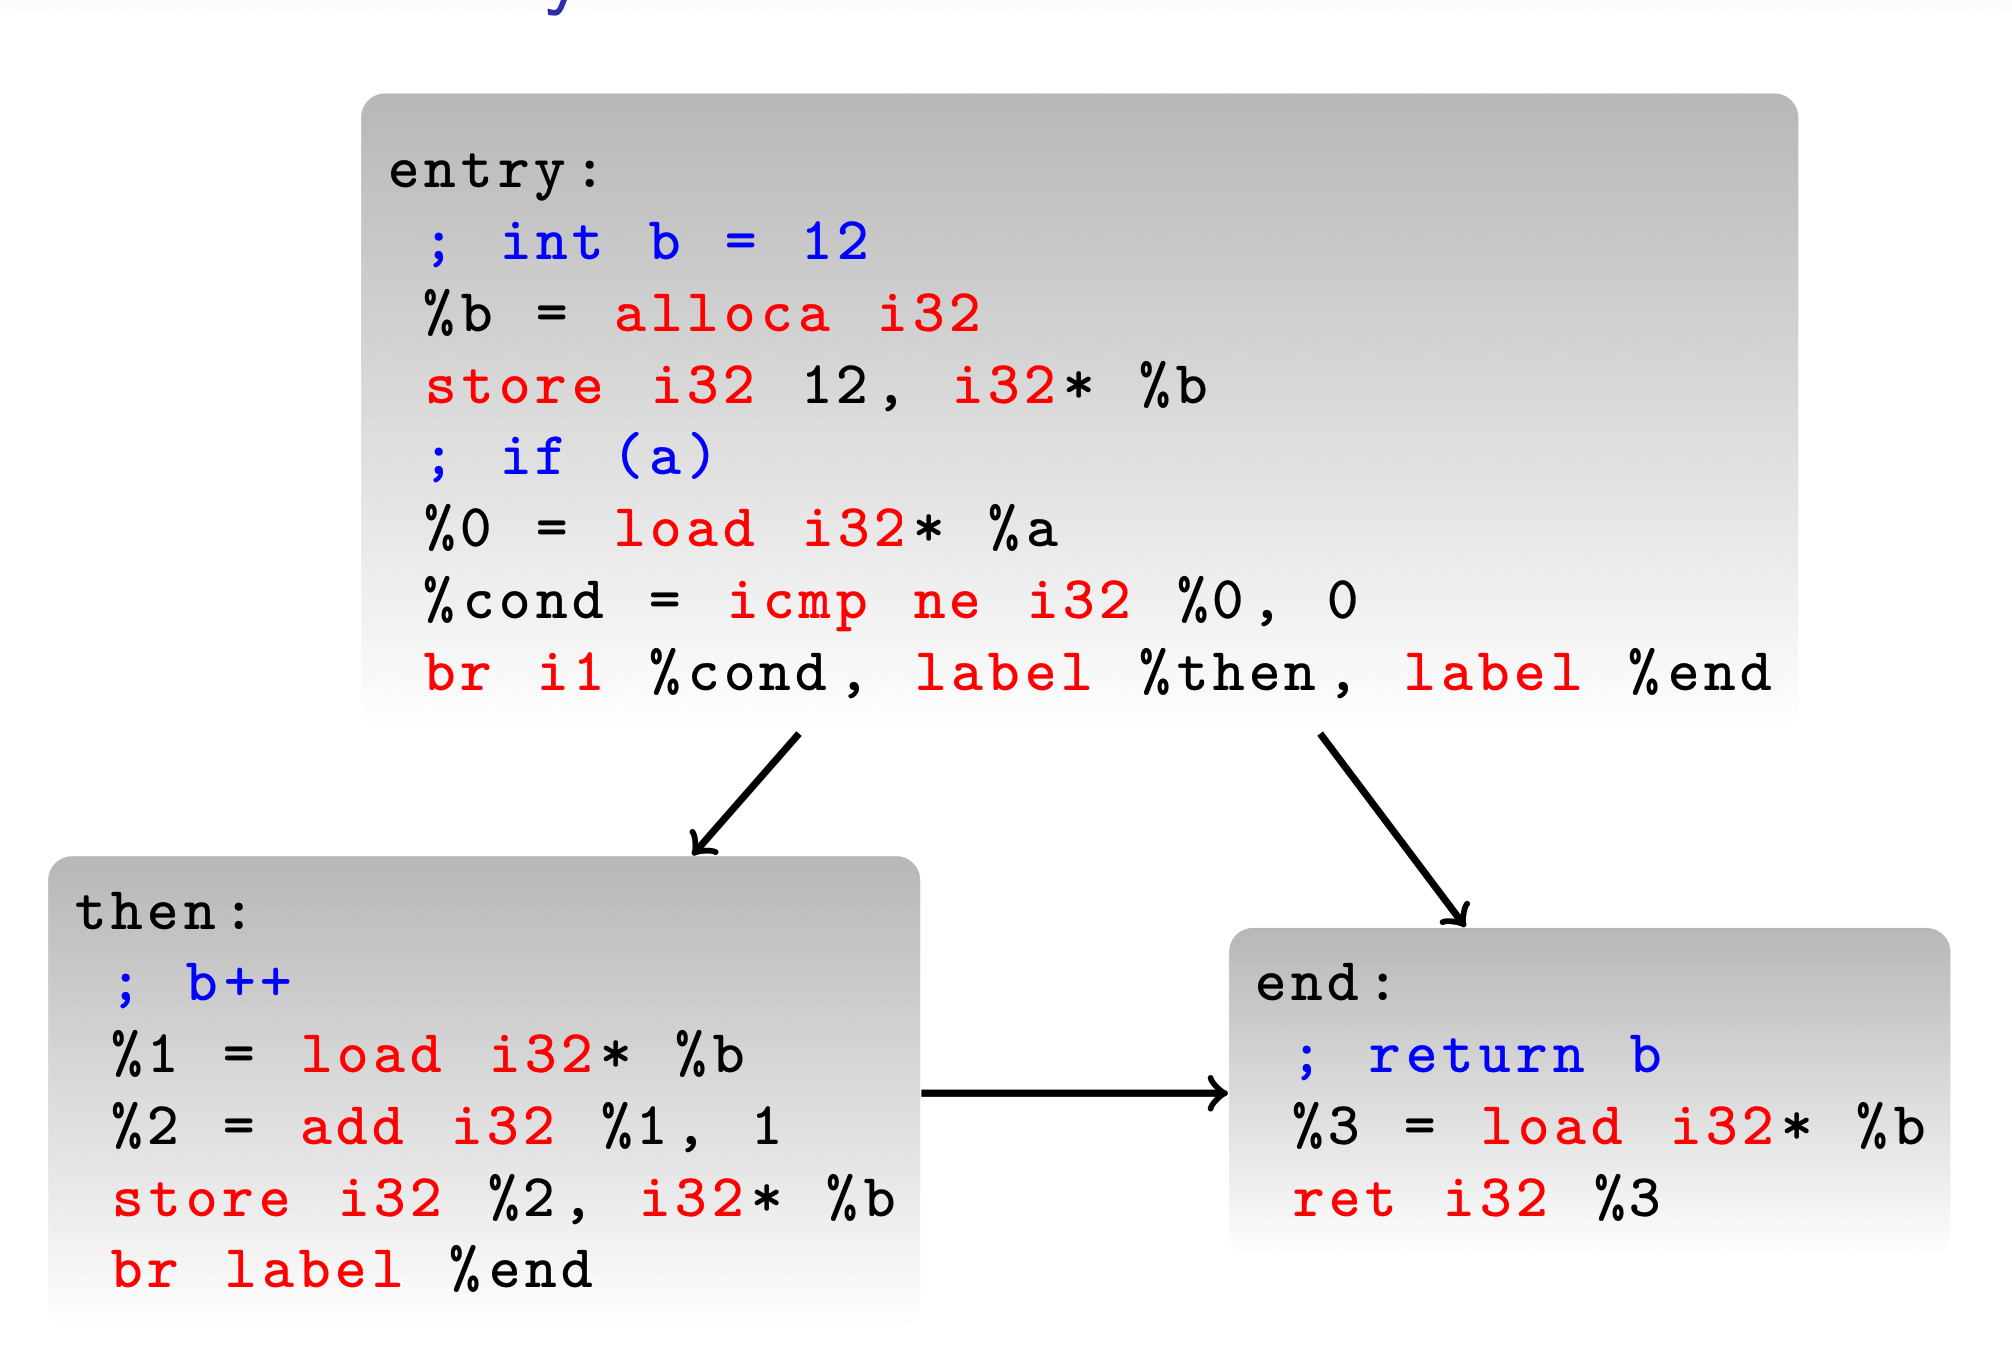
\includegraphics[height=6cm]{img/llvm_compiled_cfg.png}
\end{center}

\subsubsection{Phi Func Insertion}
% TODO
\subsection{Why Select?}
We have to select which machine instruction to generate, different ISAs have different memory models. Also, for the best performance, we have to make instruction scheduling and selection.
\begin{center}
  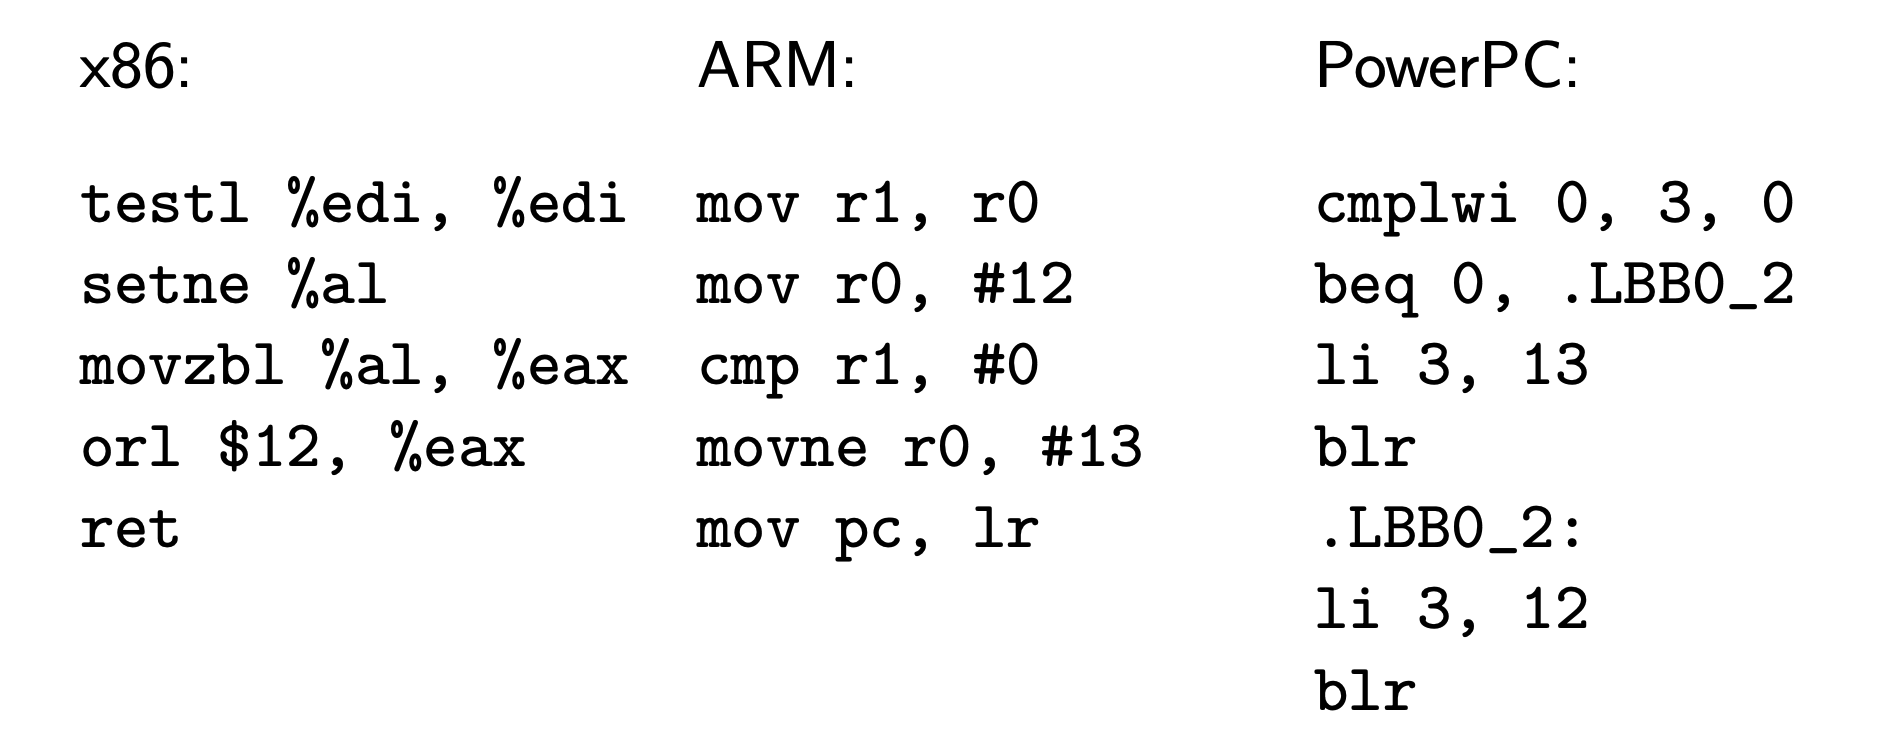
\includegraphics[width=6cm]{img/llvm_arch_diff.png}
\end{center}

\subsection{Functions}
\begin{enumerate}
  \item LLVM functions contain at least one basic block
  \item Arguments are registers and are explicitly typed
  \item Registers are valid only within a function scope
\end{enumerate}
\begin{minted}[mathescape, linenos]{llvm}
@hello = private constant [i3 x i8] c"Hello world!\00"
define i32 @main(i32 %argc, i8** %argv) {
entry:
  %0 = getelementptr [13 x i8]* @hello, i32 0, i32 0
  call i32 @puts(i8* %0)
  ret i32 0  
}
\end{minted}
\subsection{Functions in Light IR}
The Function is defined as
\begin{minted}[mathescape, linenos]{c++}
class Function : public Value {
  public:
      Function(FunctionType *ty, const string &name, Module *parent);
      ~Function() = default;
  
      static Function *create(FunctionType *ty, const string &name, Module *parent);
      static Function *create(bool is_ctor, FunctionType *ty, const string &name, Module *parent);
  
      FunctionType *get_function_type() const;
  
      Type *get_return_type() const;
  
      void add_basic_block(BasicBlock *bb);
  
      unsigned get_num_of_args() const;
      unsigned get_num_basic_blocks() const;
  
      Module *get_parent() const;
  
      list<Argument *>::iterator arg_begin() { return arguments_.begin(); }
      list<Argument *>::iterator arg_end() { return arguments_.end(); }
  
      void remove(BasicBlock *bb);
      BasicBlock *get_entry_block() { return *basic_blocks_.begin(); }
  
      list<BasicBlock *> &get_basic_blocks() { return basic_blocks_; }
      list<Argument *> &get_args() { return arguments_; }
  
      bool is_declaration() { return basic_blocks_.empty(); }
  
      void set_instr_name();
      string print() override;
      string print_method(Class *method_);
      string print_args();
      bool is_ctor = false;
  
  private:
      void build_args();
  
  private:
      list<BasicBlock *> basic_blocks_; /* basic blocks */
      list<Argument *> arguments_; /* arguments */
      Module *parent_;
      unsigned seq_cnt_;
  };
\end{minted}
First, define a function using \texttt{FuncDef} visitor pattern, and then add it to the scope finder. Just call using \texttt{builder->create\_call()} to the found previously defined function.
\begin{minted}[mathescape, linenos]{llvm}
define void @$crunch(%$.list$prototype_type* %arg0) {
 
 label1:
   %op2 = alloca i32
   %op3 = alloca %$class.anon_make_z, align 4
   %op4 = getelementptr %$class.anon_make_z, %$class.anon_make_z* %op3, i32 0, i32 0
   store i32* %op2, i32** %op4
   %op5 = getelementptr %$class.anon_make_z, %$class.anon_make_z* %op3, i32 0, i32 1
   store %$.list$prototype_type* %arg0, %$.list$prototype_type** %op5
   call void @$crunch.make_z(%$class.anon_make_z* %op3)
   %op6 = load i32, i32*@x
   br label %label7
   
 label7:                                                ; preds = %label1, %label13
   %op8 = phi i32 [ %op6, %label1 ], [ %op11, %label13 ]
   %op9 = icmp ne i32 %op6, %op8
   %op10 = getelementptr i32, i32* %op2, i32 %op8
   %op11 = add i32 %op8, 1
   %op12 = load i32, i32* %op10
   br label %label13
   
   label13:                                                ; preds = %label7
     br  i1 %op9, label %label7, label %label14
     
   label14:                                                ; preds = %label13
     ret void
}
define void @$crunch.make_z(%$class.anon_make_z* %arg0) {
     
   label1:
     %op2 = getelementptr %$class.anon_make_z, %$class.anon_make_z* %arg0, i32 0, i32 0
     %op3 = getelementptr %$class.anon_make_z, %$class.anon_make_z* %arg0, i32 0, i32 1
     %op4 = load %$.list$prototype_type*, %$.list$prototype_type** %op3
     %op5 = alloca i32
     store i32 0, i32* %op5
     %op6 = bitcast %$.list$prototype_type* %op4 to %$union.len*
     %op7 = call i32 @$len(%$union.len* %op6)
     br label %label8
     
   label8:                                                ; preds = %label1, %label17
     %op9 = phi i32 [ %op7, %label1 ], [ %op12, %label17 ]
     %op10 = icmp ne i32 %op7, %op9
     %op11 = getelementptr %$.list$prototype_type, %$.list$prototype_type* %op4, i32 0, i32 4
     %op12 = add i32 %op9, 1
     %op13 = load %$union.conslist*, %$union.conslist** %op11
     %op14 = bitcast %$union.conslist* %op13 to i32*
     %op15 = getelementptr i32, i32* %op14, i32 %op9
     %op16 = load i32, i32* %op15
     br label %label17
     
   label17:                                                ; preds = %label8
     br  i1 %op10, label %label8, label %label18
     
   label18:                                                ; preds = %label17
     ret void
}
\end{minted}

\subsection{The Most Important LLVM Classes}

\begin{enumerate}
  \item Module - A compilation unit.
  \item Function - Can you guess?
  \item BasicBlock - a basic block
  \item GlobalVariable (I hope it's obvious)
  \item IRBuilder - a helper for creating IR
  \item Type - superclass for all LLVM concrete types
  \item ConstantExpr - superclass for all constant expressions
  \item PassManagerBuilder - Constructs optimization pass sequences to run
  \item ExecutionEngine - Interface to the JIT compiler

\end{enumerate}

\subsection{Writing A Simple Pass}
\begin{enumerate}
  \item Memoise an expensive library call
  \item Call maps a string to an integer (e.g. string intern function) • Mapping can be expensive.
  \item Always returns the same result.
\end{enumerate}

\subsection{Selection DAG}
\begin{enumerate}
  \item DAG defining operations and dependencies
  \item Legalisation phase lowers IR types to target types
        \begin{enumerate}
          \item Arbitrary-sized vectors to fixed-size
          \item Float to integer and softfloat library calls
        \end{enumerate}

  \item DAG-to-DAG transforms simplify structure
  \item Code is still (more or less) architecture independent at this
        point
  \item Some peephole optimizations happen here
\end{enumerate}

\begin{center}
  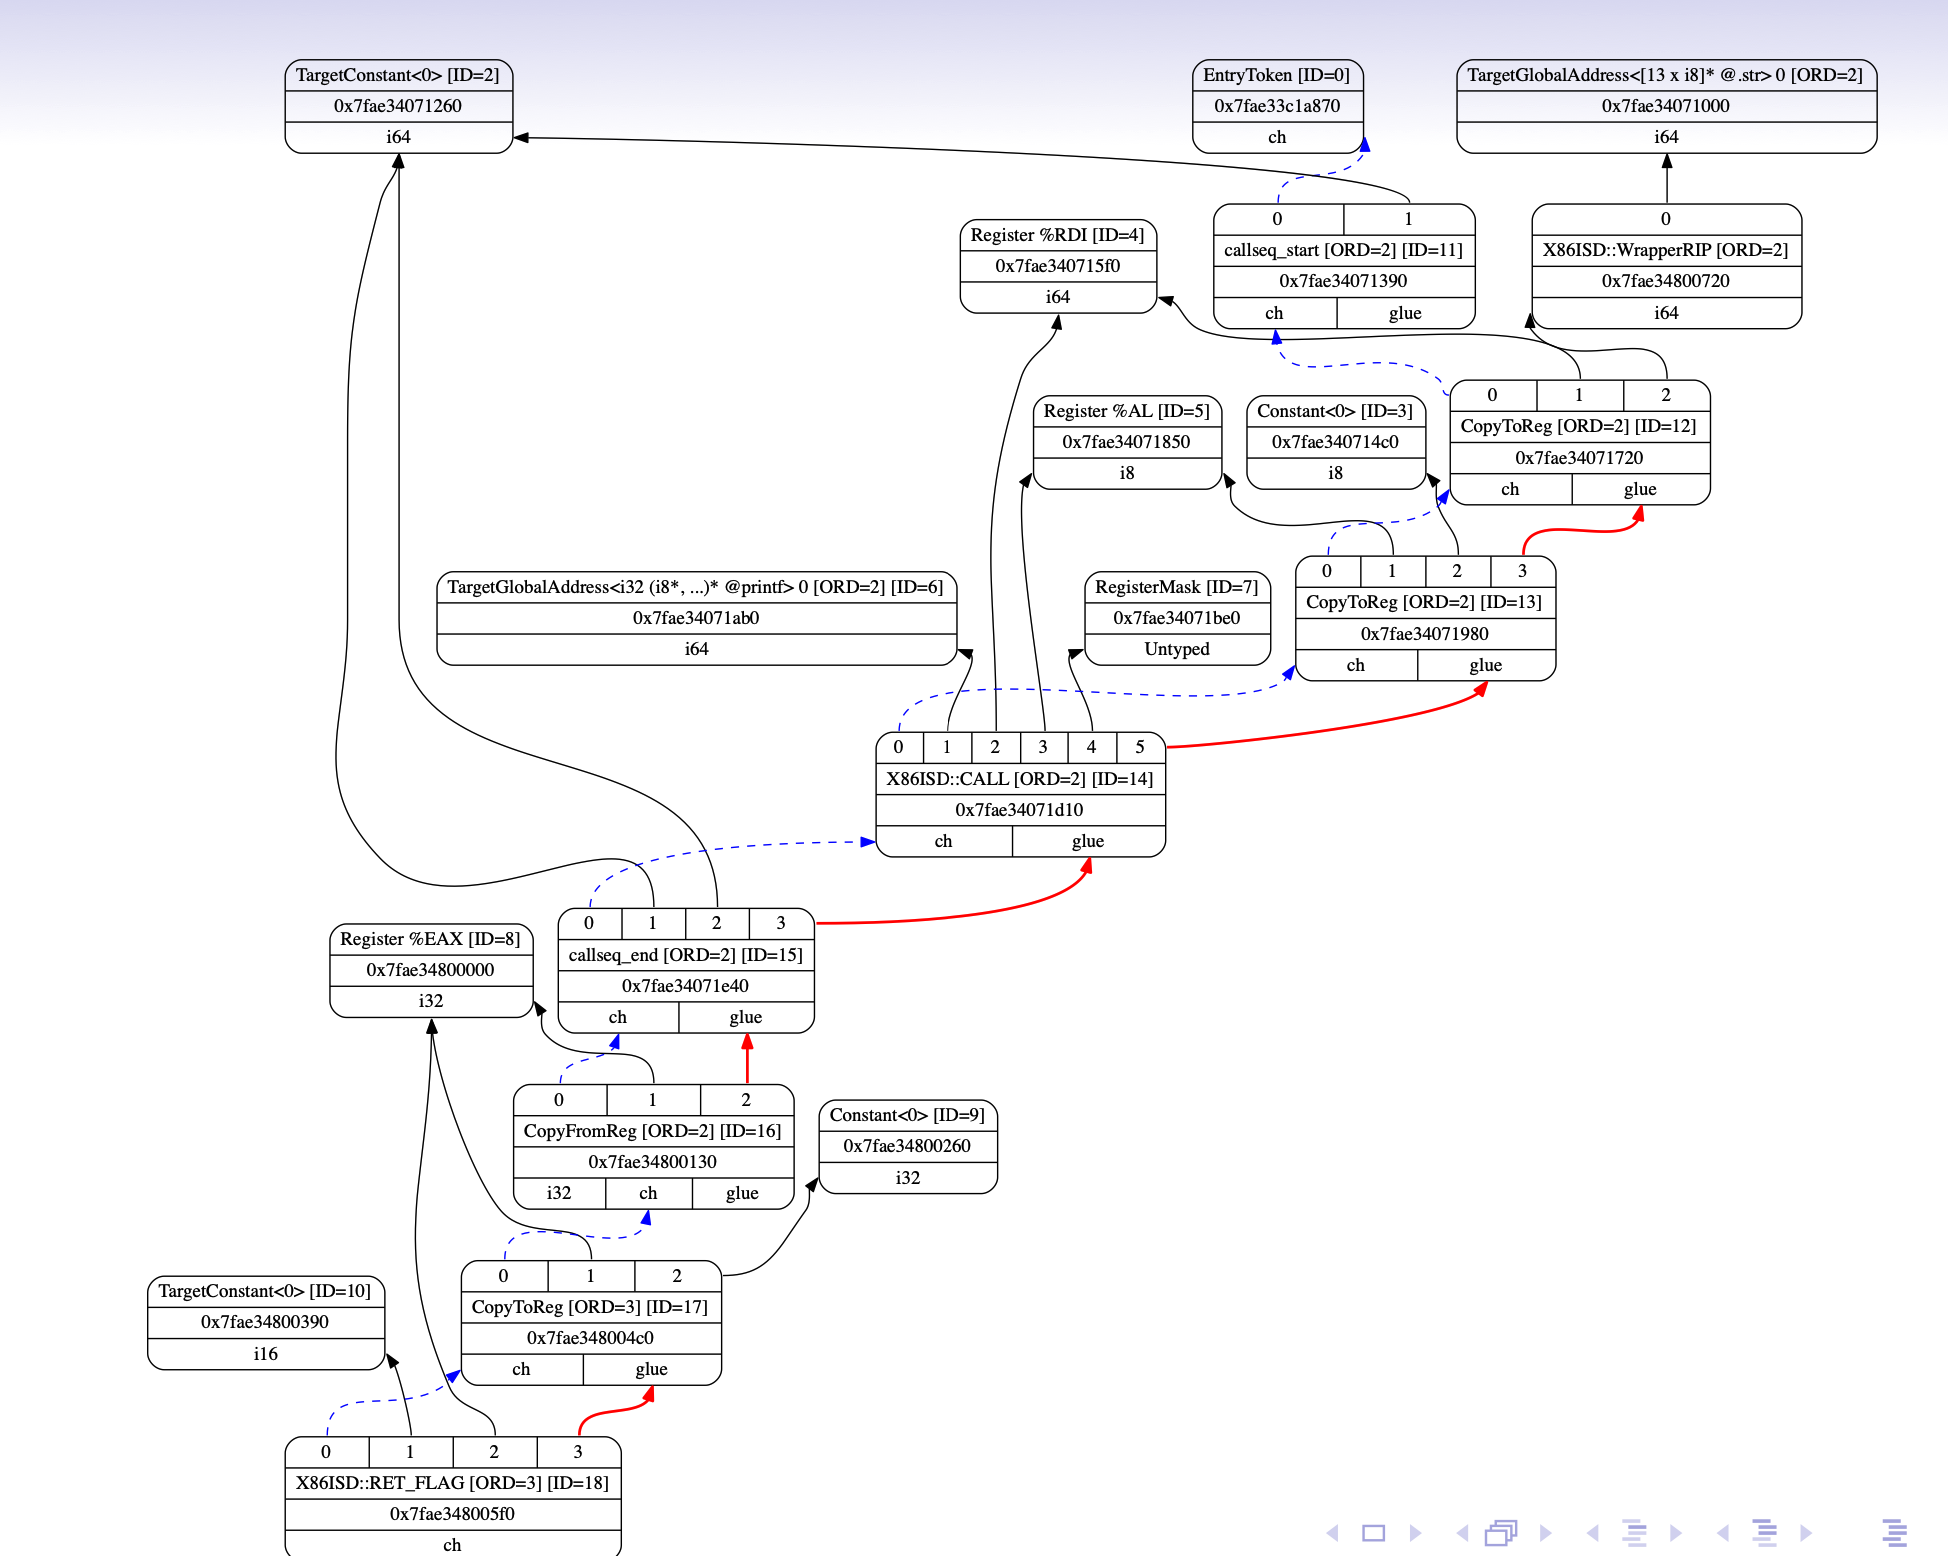
\includegraphics[height=12cm]{img/llvm_peephole.png}
\end{center}

\printbibliography
\end{document}
